\documentclass[../main.tex]{subfiles}
\LoadClass[a4paper,12pt]{article}
\documentclass{article}

%%%%%%%%%%%%%%%%%%%%%%%%%%%%%%%
%     import des packages     %
%%%%%%%%%%%%%%%%%%%%%%%%%%%%%%%
\usepackage[export]{adjustbox}
\usepackage{algorithm}
\usepackage{algorithmic}
\usepackage{amsmath,amsfonts,amssymb}
\usepackage{anyfontsize}
\usepackage{array}
\usepackage[english]{babel}
\usepackage{colortbl}
\usepackage{comment}
\usepackage{cclicenses}
\usepackage{eqnarray}
\usepackage{eso-pic}
\usepackage{dirtree}
\usepackage{fancybox}
\usepackage{fancyhdr}
\usepackage{float}
\usepackage[T1]{fontenc} 
\usepackage{forest}
\usepackage{fourier-orns}
\usepackage{gensymb}
\usepackage{geometry}
\usepackage{glossaries}
\usepackage{graphicx}
\usepackage{hyperref}
\usepackage{ifthen}
\usepackage{import}
\usepackage{indentfirst}
\usepackage[utf8]{inputenc}
\usepackage{lastpage}
\usepackage{libertine}
\usepackage{lipsum}
\usepackage{listings}
\usepackage{mathtools}
\usepackage{mdframed}
\usepackage{multicol}
\usepackage{pdfpages}
\usepackage{pifont}
\usepackage{stmaryrd}
\usepackage{subcaption}
\usepackage{subfiles}
\usepackage{tabularx}
% \usepackage{tcolorbox}
\usepackage[most]{tcolorbox}
\usepackage{textcomp}
\usepackage{ulem}
\usepackage{wrapfig}

%%%%%%%%%%%%%%%%%%%%%%%%%%%%%%%%%%%%%%%%%%%%%%%%%%%%%%%%%
%    Renseigner les titres et variables importantes     %
%%%%%%%%%%%%%%%%%%%%%%%%%%%%%%%%%%%%%%%%%%%%%%%%%%%%%%%%%
\newcommand{\titre}{Multi-robot coordination}
\newcommand{\soustitre}{Autonomous exploration of gallery networks}
\newcommand{\sujet}{Engineering Graduation Project}
\newcommand{\sujets}{Seatech 3A - MOCA}
\newcommand{\auteur}{Fabien MATHÉ}
\newcommand{\referent}{M. Mehmet ERSOY}
\newcommand{\reportdate}{\date}

\newcommand{\partA}{State of the art}
\newcommand{\partB}{Partie 2}
\newcommand{\partC}{Partie 3}
\newcommand{\partD}{Partie 4}
\newcommand{\partE}{Partie 5}

%%%%%%%%%%%%%%%%%%%
%     BOOLEEN     %
%%%%%%%%%%%%%%%%%%%

% Création des boolean
\newboolean{abst}
\newboolean{thx}
\newboolean{contents}
\newboolean{introduction}
\newboolean{pt2}
\newboolean{pt3}
\newboolean{pt4}
\newboolean{pt5}
\newboolean{conclusion}
\newboolean{perspectives}
\newboolean{glossaire}
\newboolean{biblio}
\newboolean{annexe}


% Renseigner si le Rapport contient un abstract
\setboolean{abst}{true}
% Renseigner si le Rapport contient des remerciements
\setboolean{thx}{true}
% Renseigner si le Rapport contient une table des matières
\setboolean{contents}{true}
% Renseigner si le Rapport contient une introduction
\setboolean{introduction}{true}
% Renseigner si le Rapport contient une partie 2
\setboolean{pt2}{true}
% Renseigner si le Rapport contient une partie 3
\setboolean{pt3}{true}
% Renseigner si le Rapport contient une partie 4
\setboolean{pt4}{true}
% Renseigner si le Rapport contient une partie 5
\setboolean{pt5}{true}
% Renseigner si le Rapport contient une introduction
\setboolean{conclusion}{true}
% Renseigner si le Rapport contient des perspectives
\setboolean{perspectives}{true}
% Renseigner si le document contient une bibliographie
\setboolean{biblio}{true} 
% Renseigner si le document contient un glossaire
\setboolean{glossaire}{false}
% Renseigner si le Rapport contient des annexes 
\setboolean{annexe}{true}


%%%%%%%%%%%%%%%%%%%%%%%%%%%%%%%%%%%%%%
%     En-têtes en pieds de pages     %
%%%%%%%%%%%%%%%%%%%%%%%%%%%%%%%%%%%%%%
\geometry{hmargin=2cm,vmargin=2.3cm}
\pagestyle{fancy}
\fancyhfoffset[]{0pt}
\setlength{\headheight}{28pt}
\lhead{
\includegraphics[height = 0.6cm]{IMAGES/logos/Logo_SeaTech_2023.png}}
% \rhead{
\includegraphics[height = 0.7cm]{IMAGES/logos/MOCA.png}}
\rhead{\textsc{\leftmark}}

% Update \rightmark with \section name
\renewcommand{\sectionmark}[1]{\markboth{#1}{#1}}


\lfoot{\auteur}
\cfoot{ }
\rfoot{Page \thepage \ / \pageref{LastPage}}

\title{\titre}
\author{\auteur}
\date{\today}

%%%%%%%%%%%%%%%%%%%%%%%%%%%%%%
%     Autre mise en page     %
%%%%%%%%%%%%%%%%%%%%%%%%%%%%%%
\numberwithin{figure}{section}
\numberwithin{table}{section}

\setcounter{tocdepth}{2} % Change to 1 to exclude subsections as well


\newcommand{\citeURL}[1]{\href{#1}{\detokenize{#1}}}

% Création du compteur d'annexes
\newcounter{annexecounter}

% Définition de la commande pour les annexes
\NewDocumentCommand{\annexe}{m}{%
    \stepcounter{annexecounter} % Incrémenter le compteur d'annexes
    \subsection*{Annexe \arabic{annexecounter} - #1} % Affichage du texte avec le numéro et le titre
	\label{sec:#1}
}

\newcommand{\tobedone}{\textcolor{red}{\LARGE \textbf{TO BE DONE}}}
\newcommand{\annexetonum}{\textcolor{red}{\LARGE \textbf{ANNEXE ...}}}

\renewcommand{\familydefault}{\sfdefault}



%%%%%%%%%%%%%%%%%%%%%%%%%%%%%%%%%
%     Mise en page des codes    %
%%%%%%%%%%%%%%%%%%%%%%%%%%%%%%%%%
\definecolor{codegreen}{rgb}{0,0.6,0}
\definecolor{codegray}{rgb}{0.5,0.5,0.5}
\definecolor{codepurple}{rgb}{0.58,0,0.82}
\definecolor{backcolour}{rgb}{0.95,0.95,0.92}

\lstdefinestyle{python}{
	backgroundcolor=\color{backcolour},
	commentstyle=\color{codegreen},
	keywordstyle=\color{blue},
	numberstyle=\tiny\color{codegray},
	stringstyle=\color{codepurple},
	basicstyle=\ttfamily\scriptsize,
	breakatwhitespace=false,
	breaklines=true,
	captionpos=b,
	keepspaces=true,
	numbers=left,
	numbersep=5pt,
	showspaces=false,
	showstringspaces=false,
	showtabs=false,
	tabsize=2
}

\lstset{style=python}
\definecolor{codegreen}{rgb}{0,0.6,0}
\definecolor{codegray}{rgb}{0.5,0.5,0.5}
\definecolor{codepurple}{rgb}{0.58,0,0.82}
\definecolor{backcolour}{rgb}{0.95,0.95,0.92}

\lstdefinestyle{cpp}{
	backgroundcolor=\color{backcolour},
	commentstyle=\color{codegreen},
	keywordstyle=\color{blue},
	numberstyle=\tiny\color{codegray},
	stringstyle=\color{codepurple},
	basicstyle=\ttfamily\scriptsize,
	breakatwhitespace=false,
	breaklines=true,
	captionpos=b,
	keepspaces=true,
	numbers=left,
	numbersep=5pt,
	showspaces=false,
	showstringspaces=false,
	showtabs=false,
	tabsize=2,
	language=C++
}

\lstset{style=cpp}

\definecolor{codegreen}{rgb}{0,0.6,0}
\definecolor{codegray}{rgb}{0.5,0.5,0.5}
\definecolor{codepurple}{rgb}{0.58,0,0.82}
\definecolor{backcolour}{rgb}{0.95,0.95,0.92}

\lstdefinestyle{fortran}{
    backgroundcolor=\color{backcolour},
    commentstyle=\color{codegreen},
    keywordstyle=\color{blue},
    numberstyle=\tiny\color{codegray},
    stringstyle=\color{codepurple},
    basicstyle=\ttfamily\scriptsize,
    breakatwhitespace=false,
    breaklines=true,
    captionpos=b,
    keepspaces=true,
    numbers=left,
    numbersep=5pt,
    showspaces=false,
    showstringspaces=false,
    showtabs=false,
    tabsize=2,
    language=[90]Fortran
}

\lstset{style=fortran}


%%%%%%%%%%%%%%%%%%%%%%%%%%%%%%%%%%%%%%%%%%%%%%%%%%%%%%%%%%%%%%%%%%%%%%%%%%%%%%%%%%%%%%%%%%%%%%%%%%%%%%%%%%%%%%%%%%%%%%%
%                                                  Début du document                                                  %
%%%%%%%%%%%%%%%%%%%%%%%%%%%%%%%%%%%%%%%%%%%%%%%%%%%%%%%%%%%%%%%%%%%%%%%%%%%%%%%%%%%%%%%%%%%%%%%%%%%%%%%%%%%%%%%%%%%%%%%

\begin{document}

%%%%%%%%%%%%%%%%%%%%%%%%%
%     Page de garde     %
%%%%%%%%%%%%%%%%%%%%%%%%%
\begin{titlepage}
	\AddToShipoutPictureBG*{
\includegraphics[width=\paperwidth,height=\paperheight]{IMAGES/PageDeGardeRapport.png}}
	\begin{figure}[H]
		\begin{subfigure}{0.45\linewidth}
				
\includegraphics[width=0.6\textwidth,left]{IMAGES/logos/Logo_SeaTech_2023.png}
		\end{subfigure}
		\hfill
		\begin{subfigure}{0.45\linewidth}
				% 
\includegraphics[width=0.6\textwidth,right]{IMAGES/logos/MOCA.png}
		\end{subfigure}
	\end{figure}

	\centering

	% Espacement vertical
	\vspace*{5cm}

	% Barres horizontales
	\makebox[0.7\linewidth]{\hrulefill}\\[0.2cm]

	% Titre encadré
	\vspace{0.5cm}
	\begin{minipage}{\textwidth}
		\centering
		{\fontsize{28}{48}\selectfont \textsc{\titre}}\\[0.2cm]

		{\fontsize{18}{48}\selectfont \textsc{\soustitre}}
	\end{minipage}
	\vspace{0.3cm}

	% Barres horizontales
	\makebox[0.8\linewidth]{\hrulefill}\\[0.2cm]

	% Espacement vertical
	\vspace{3cm}

	% Description
		\large{\Large \textbf{\sujet}}\\
		\large{\textbf{\sujets}}\\

		\vspace{0.5cm}
		\large{\textbf{\reportdate}}

	\vspace{2cm}

	\begin{minipage}{0.20\textwidth}

	\end{minipage}
	\hfill
	\begin{minipage}{0.35\textwidth}
		\begin{flushleft}
			Auteur : \\
			\auteur
		\end{flushleft}
	\end{minipage}
	\begin{minipage}{0.09\textwidth}
		% Section vide pour espacement optimal
	\end{minipage}
	\hfill
 	\begin{minipage}{0.3\textwidth}
		\begin{flushleft}
			Enseignant : \\
			\referent

		\end{flushleft}
	\end{minipage}


\end{titlepage}

\ClearShipoutPictureBG

\newpage

\renewcommand{\thepage}{}

\renewcommand{\thepage}{\arabic{page}}
\renewcommand{\thesection}{\Roman{section}}

%%%%%%%%%%%%%%%%%%
%     Résumé     %
%%%%%%%%%%%%%%%%%%
\ifthenelse{\boolean{abst}}{
	\addcontentsline{toc}{section}{\protect\numberline{}Résumé}%
	\subfile{SECTIONS/1resume}

	\newpage
}

%%%%%%%%%%%%%%%%%%%%%%%%%
%     Remerciements     %
%%%%%%%%%%%%%%%%%%%%%%%%%
\ifthenelse{\boolean{thx}}{
	\addcontentsline{toc}{section}{\protect\numberline{}Remerciements}%
	\subfile{SECTIONS/2remerciements}

	\newpage
}

%%%%%%%%%%%%%%%%%%%%%%%%%%%%
%     Plan du document     %
%%%%%%%%%%%%%%%%%%%%%%%%%%%%

\ifthenelse{\boolean{contents}}{
	\vfill
	\tableofcontents
	\vfill
	
	\newpage
}

%%%%%%%%%%%%%%%%%%%%%%%%
%     INTRODUCTION     %
%%%%%%%%%%%%%%%%%%%%%%%%
\ifthenelse{\boolean{introduction}}
{
	\addcontentsline{toc}{section}{\protect\numberline{}Introduction}%
	\section*{Introduction}

	\markboth{Introduction}{Introduction} % Manually update \rightmark for section*
	\subfile{SECTIONS/3introduction}


	\newpage
}


%%% PARTIE 1 %%%
\section{\partA}
\subfile{SECTIONS/part1}

%%% PARTIE 2 %%%
\newpage
\ifthenelse{\boolean{pt2}}
{
	\section{\partB}
	\subfile{SECTIONS/part2}
	
	\newpage
}
	
	
%%% PARTIE 3 %%%
\ifthenelse{\boolean{pt3}}
{
	\section{\partC}
	\subfile{SECTIONS/part3}
	
	\newpage
}
	
	
%%% PARTIE 4 %%%
\ifthenelse{\boolean{pt4}}
{
	\section{\partD}
	\subfile{SECTIONS/part4}
	
	\newpage
}
	
%%% PARTIE 5 %%%
\ifthenelse{\boolean{pt5}}{
	\section{\partE}
	\subfile{SECTIONS/part5}

	\newpage
}
		
%%%%%%%%%%%%%%%%%%%%%%
%     CONCLUSION     %
%%%%%%%%%%%%%%%%%%%%%%
\ifthenelse{\boolean{perspectives}}
{
	\addcontentsline{toc}{section}{\protect\numberline{}Conclusion}%
	\section*{Conclusion}
	\markboth{Introduction}{Introduction} % Manually update \rightmark for section*

	\subfile{SECTIONS/Wconclusion}

	\newpage
}



\ifthenelse{\boolean{perspectives}}
{
	\section*{Perspectives}
	\addcontentsline{toc}{section}{\protect\numberline{}Perspectives}
	\subfile{SECTIONS/Xperspectives}
	
	\newpage 
}

%%%%%%%%%%%%%%%%%%%%%%%%%
%     Bibliographie     %
%%%%%%%%%%%%%%%%%%%%%%%%%

\ifthenelse{\boolean{biblio}}
{
	\addcontentsline{toc}{section}{\protect\numberline{}References}
	% \bibliographystyle{unsrt}
	\bibliographystyle{IEEEtran}
	\footnotesize{\bibliography{BIBLIOGRAPHY/bib.bib}}

	\newpage
}


%%%%%%%%%%%%%%%%%%%%%
%     Glossaire     %
%%%%%%%%%%%%%%%%%%%%%
\normalsize
\ifthenelse{\boolean{glossaire}}
{
	\section*{Glossaire}
	\makeglossaries
	\printglossaries
	\addcontentsline{toc}{section}{\protect\numberline{}Glossaire}%
	\subfile{SECTIONS/Yglossaire}
	
	\newpage
}

%%%%%%%%%%%%%%%%%%%
%     Annexes     %
%%%%%%%%%%%%%%%%%%%
\ifthenelse{\boolean{annexe}}
{
	\section*{Annexes}
	\addcontentsline{toc}{section}{\protect\numberline{}Annexes}%
	\subfile{SECTIONS/Zannexes}
}


\end{document}


\begin{document}

To further develop this work, I aim to explore another way to acheive optimal path. As seen earlier, global path optimization was not entirely successful. To address this, I simplified the problem and focused on a new approach that frames it as a control problem from both a mathematical and empirical perspective. Both aspects are still under development and must be implemented in the simulator later.

\subsection*{Local Path Theory}

\subsubsection*{First Approach: Mathematical Optimization}

In this section, we seek to determine the optimal control commands that allow the robot to navigate toward a local waypoint without collisions while adhering to its physical constraints.

\vspace{1em}

Here, "optimal" refers to minimizing energy consumption when moving from point A to point B. Since the robot operates with DC motors, power consumption is proportional to voltage (which affects rotation speed) and current (which influences torque). Assuming a flat surface and constant torque, current remains unchanged, meaning energy consumption is primarily determined by wheel speed. The energy expenditure for movement is defined as:

\begin{equation}
    E(T) = \int_{0}^{T} \| \omega(t) \| \, dt
\end{equation}

where

\begin{equation}
    \| \omega (t) \| = \sqrt{\omega_L^{2}(t) + \omega_R^{2}(t)}
\end{equation}

and

\begin{equation}
    \omega_{L, R} \,:\, \mathbb{R}_+ \longrightarrow [-\omega_{max}, \omega_{max}]
\end{equation}

Two constraints must be satisfied: the robot's initial position $X(0)$ must match its current position $X_R$, and its final position $X(T)$ must correspond to the waypoint $X_{WP}$.

\vspace{1em}

In \autoref{sec:robot_model}, we derived the system dynamics as $\dot{X} = F(\omega)$.

\vspace{1em}

The goal is then to optimize $E(T)$.

\vspace{1em}

\paragraph{Note:} If the current were not constant, energy consumption would depend on the terrain characteristics. In this case, energy would be defined as:

\begin{equation}
    \tilde{E}(T) = \int_{0}^{T} \| U(t) I(t) \| dt
\end{equation}

where $U(t)$ and $I(t)$ vary based on environmental conditions. This would significantly increase the problem's complexity.

The challenge remains identical to that in global path optimization: How can we ensure that $X(T) = X_{WP}$?

\subsubsection*{Second Approach: Empirical Optimization}

The second approach involves determining the set of all possible maximal paths that the robot can follow within a given time frame. By reversing the problem, we can infer the optimal control commands needed to reach the waypoint efficiently.

Initially, I focus on identifying the maximal paths using stochastic methods, see \autoref{fig:stocha_path}. Then, I compute all feasible path combinations for a given number of distinct control inputs, see \autoref{fig:empir_path}. This approach provides a data-driven way to refine the navigation strategy, complementing the theoretical optimization.

\begin{figure}[H]
	\centering
	\begin{subfigure}[b]{0.45\textwidth}
		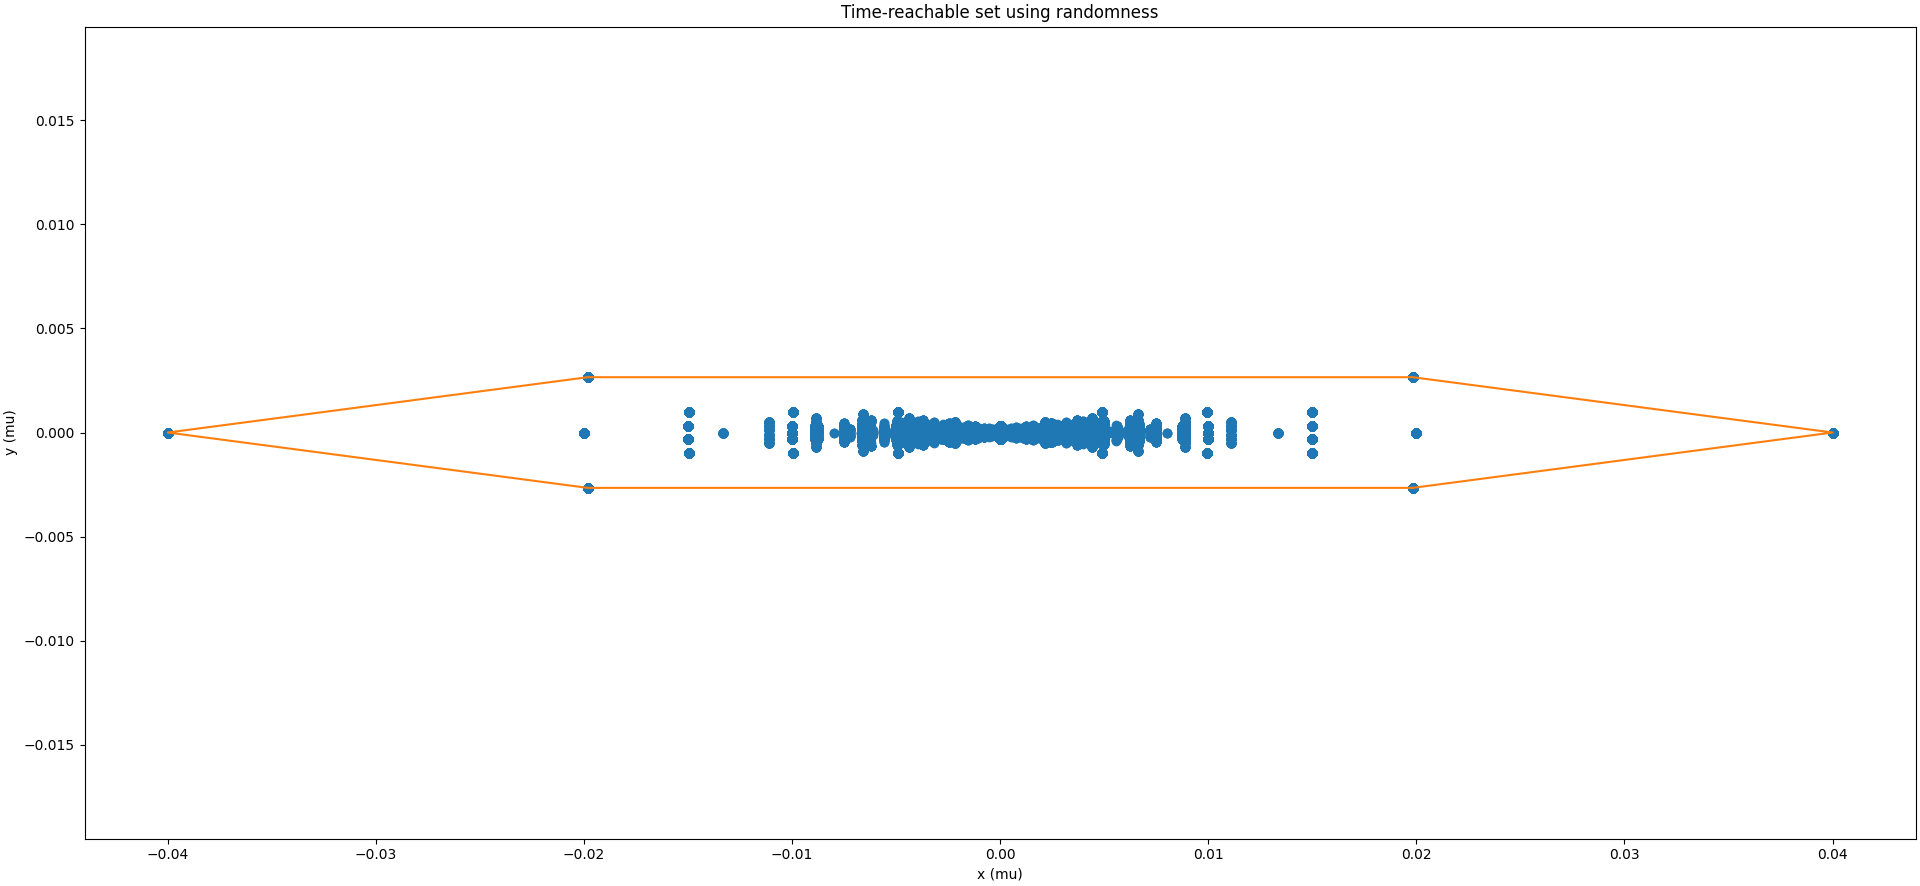
\includegraphics[width=\textwidth]{IMAGES/perspectives/random.png}
		\caption{Stochastic Path}
		\label{fig:stocha_path}
	\end{subfigure}
	\hfill
	\begin{subfigure}[b]{0.45\textwidth}
		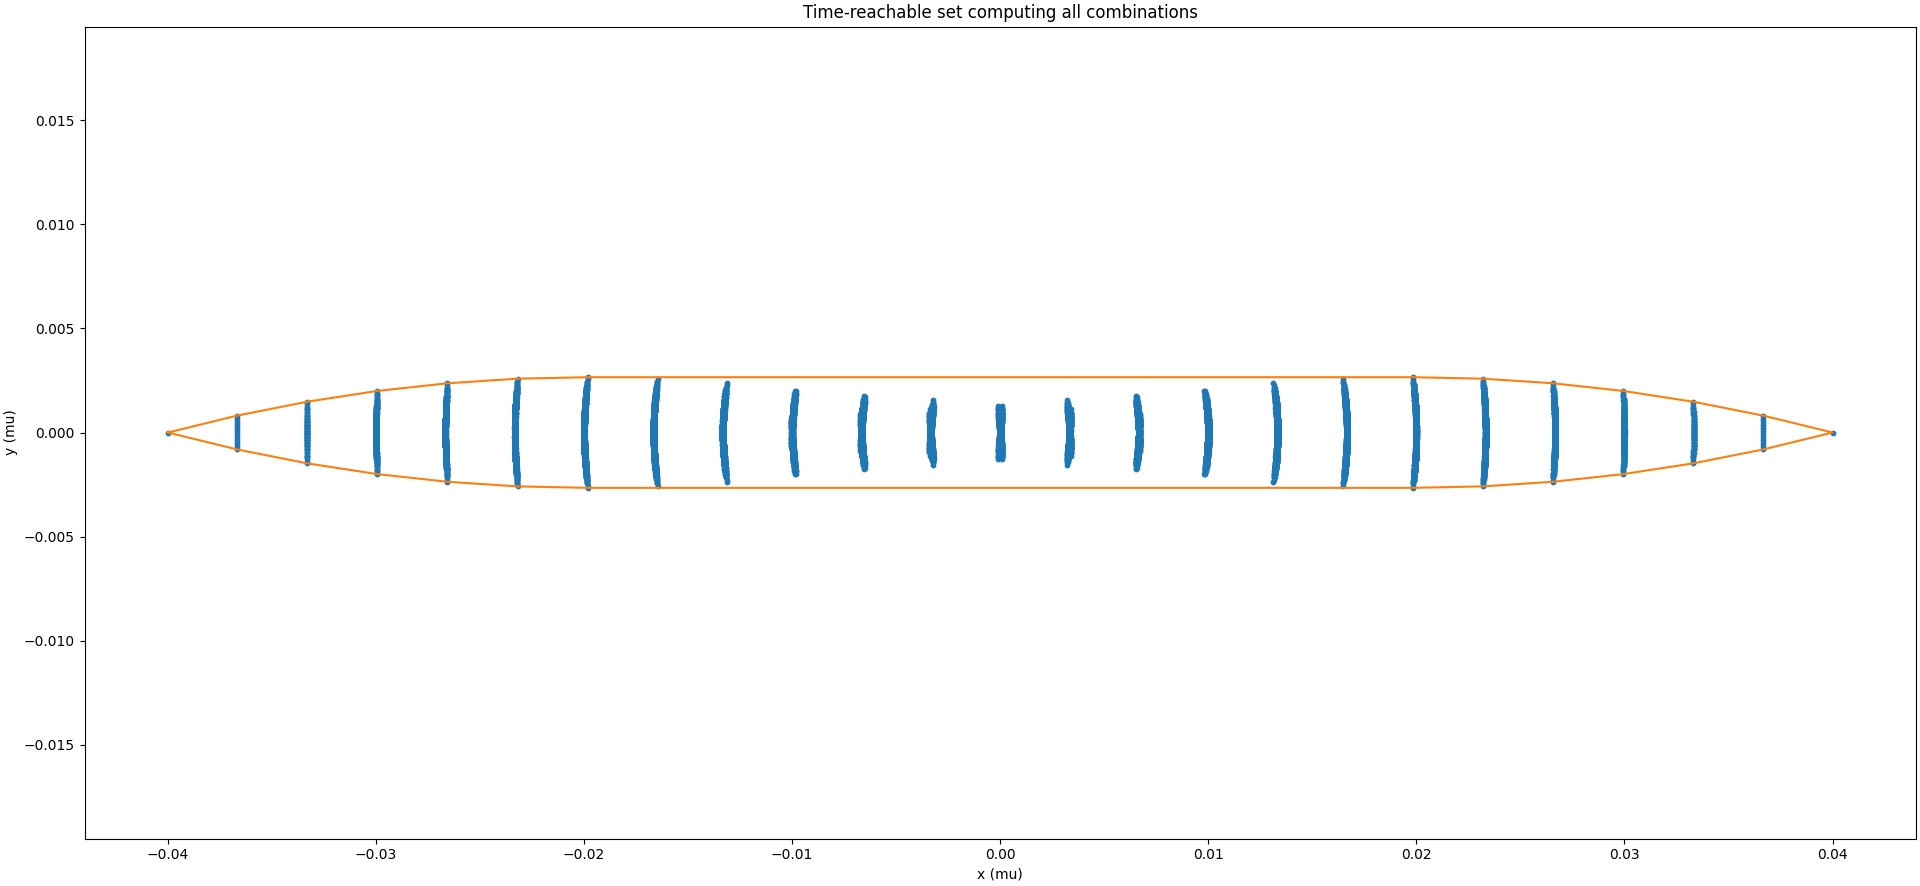
\includegraphics[width=\textwidth]{IMAGES/perspectives/empiric.png}
		\caption{Empirical Path}
		\label{fig:empir_path}
	\end{subfigure}
	\caption{Comparison of Stochastic and Empirical Path Optimization Approaches}
	\label{fig:path_optimization}
\end{figure}

Results were better simulating all combinations possible.

\subsection*{ROS Implementation}
Possible future work includes implementing the simulator within a Robot Operating System (ROS) architecture, integrated with RViz or Gazebo for visualization and testing. ROS is a middleware that provides a flexible framework for developing robotic applications by offering tools, libraries, and conventions to simplify communication between different robotic components. 

\vspace{1em}

By implementing the simulator in ROS, we can enhance modularity, allowing seamless integration of additional sensors, actuators, and real-world robotic hardware. Gazebo, as a high-fidelity physics simulator, would enable realistic testing of the robot's movement and interaction with dynamic environments, while RViz would facilitate real-time visualization of sensor data and path planning.

\vspace{1em}

Moreover, integrating ROS would allow for better compatibility with existing robotic platforms, making it easier to transition from simulation to real-world deployment. Future work could also explore ROS2 for improved performance, scalability, and real-time capabilities, further enhancing multi-robot coordination and communication.

\vspace{1em}

The energy consumption shoulf also be implemented to account for the robot's real-time power usage, considering factors such as motor efficiency, battery limitations, and terrain characteristics.

\subsection*{PhD oppening}
All these open areas in my work will be essential components of my future research within the framework of my PhD. The main objective will be to design optimal trajectory planning algorithms for the recovery of underwater drone swarms. This work represents the first step into the world of robotics and mathematics research, a field I will continue to explore and develop during my PhD, which is currently in the process of securing funding.


\end{document}